\RequirePackage{currfile}
\documentclass[12pt]{beamer}
\usepackage[utf8]{inputenc}
\usepackage[spanish]{babel}
\usepackage{standalone}
\usepackage{color}
\usepackage{siunitx}
\usepackage{hyperref}
%\hypersetup{colorlinks,linkcolor=,urlcolor=blue}
%\hypersetup{colorlinks,urlcolor=blue}
\usepackage{xcolor,soul}
\usepackage{etoolbox}
\usepackage{amsmath}
\usepackage{amsthm}
\usepackage{physics}
\usepackage{multicol}
\usepackage{bookmark}
\usepackage{longtable}
\usepackage{listings}
\lstset{
basicstyle=\ttfamily,
columns=flexible,
breaklines=true
}
\usepackage{graphicx}
\usepackage{tikz}
\usetikzlibrary{matrix,backgrounds}
\usepackage[autostyle,spanish=mexican]{csquotes}
\usepackage[os=win]{menukeys}
\usepackage{pifont}
\usepackage{pbox}
\usepackage{caption}
\captionsetup{font=scriptsize,labelfont=scriptsize}

\definecolor{ao}{rgb}{0.0, 0.5, 0.0}
\definecolor{bisque}{rgb}{1.0, 0.89, 0.77}
\definecolor{amber}{rgb}{1.0, 0.75, 0.0}
\definecolor{armygreen}{rgb}{0.29, 0.33, 0.13}
\definecolor{alizarin}{rgb}{0.82, 0.1, 0.26}
\definecolor{cadetblue}{rgb}{0.37, 0.62, 0.63}
\definecolor{deepblue}{rgb}{0,0,0.5}
\definecolor{brown}{rgb}{0.59, 0.29, 0.0}
\definecolor{OliveGreen}{rgb}{0,0.25,0}

\definecolor{Code}{rgb}{0,0,0}
\definecolor{Keywords}{rgb}{255,0,0}
\definecolor{Strings}{rgb}{255,0,255}
\definecolor{Comments}{rgb}{0,0,255}
\definecolor{Numbers}{rgb}{255,128,0}


\newcommand*{\TitleParbox}[1]{\parbox[c]{1.75cm}{\raggedright #1}}%

%\usepackage[sfdefault]{roboto}  %% Option 'sfdefault' only if the base font of the document is to be sans serif

\renewcommand{\arraystretch}{1.5}
\renewcommand{\rmdefault}{cmr}% cmr = Computer Modern Roman
\usefonttheme[onlymath]{serif}

\newcommand{\python}{\texttt{python}}
\newcommand{\textoazul}[1]{\textcolor{blue}{#1}}
\newcommand{\azulfuerte}[1]{\textcolor{blue}{\textbf{#1}}}
\newcommand{\funcionazul}[1]{\textcolor{blue}{\textbf{\texttt{#1}}}}

\newcounter{saveenumi}
\newcommand{\seti}{\setcounter{saveenumi}{\value{enumi}}}
\newcommand{\conti}{\setcounter{enumi}{\value{saveenumi}}}

\linespread{1.5}
\beamertemplatenavigationsymbolsempty
\usefonttheme{professionalfonts}
%\usefonttheme{serif}
\DeclareGraphicsExtensions{.pdf,.png,.jpg}
\renewcommand {\arraystretch}{1.25}
\mode<presentation>
{
  \usetheme{Warsaw}
  \setbeamertemplate{headline}{}
  %\useoutertheme{infolines}
  \useoutertheme{default}
  \setbeamercovered{invisible}
  % or whatever (possibly just delete it)
  \setbeamertemplate{section in toc}[sections numbered]
  \setbeamertemplate{subsection in toc}[subsections numbered]
  \setbeamertemplate{subsection in toc}{\leavevmode\leftskip=3.2em\rlap{\hskip-2em\inserttocsectionnumber.\inserttocsubsectionnumber}\inserttocsubsection\par}
  \setbeamercolor{section in toc}{fg=blue}
  \setbeamercolor{subsection in toc}{fg=blue}
  \setbeamercolor{frametitle}{fg=yellow}

  \setbeamertemplate{footline} 
{
  \leavevmode%
  \hbox{%
  \begin{beamercolorbox}[wd=.333333\paperwidth,ht=2.25ex,dp=1ex,center]{author in head/foot}%
    \usebeamerfont{author in head/foot}\insertsection
  \end{beamercolorbox}%
  \begin{beamercolorbox}[wd=.333333\paperwidth,ht=2.25ex,dp=1ex,center]{title in head/foot}%
    \usebeamerfont{title in head/foot}\textcolor{yellow}{\insertsubsection}
  \end{beamercolorbox}%
  \begin{beamercolorbox}[wd=.333333\paperwidth,ht=2.25ex,dp=1ex,right]{date in head/foot}%
    \usebeamerfont{date in head/foot}\insertshortdate{}\hspace*{2em}
    \insertframenumber{} / \inserttotalframenumber\hspace*{2ex} 
  \end{beamercolorbox}}%
  \vskip0pt%
}
}
\makeatother

\makeatletter
\patchcmd{\beamer@sectionintoc}
  {\vfill}
  {\vskip\itemsep}
  {}
  {}
\makeatother

% \makeatletter
% \patchcmd{\hyper@link@}
%   {{\Hy@tempb}{#4}}
%   {{\Hy@tempb}{\ul{#4}}}
%   {}{}
% \makeatother

\DeclareCaptionFont{white}{\color{white}}
\DeclareCaptionFormat{listing}{\colorbox{gray}{\parbox{0.99\textwidth}{#1#2#3}}}
\captionsetup[lstlisting]{format=listing,labelfont=white,textfont=white}
\renewcommand{\lstlistingname}{Código}

\lstdefinestyle{codigopython}{%
  language=Python,                % choose the language of the code
  %basicstyle=\footnotesize\small,       % the size of the fonts that are used for the code
  numbers=left,                   % where to put the line-numbers
  numberstyle=\scriptsize,      % the size of the fonts that are used for the line-numbers
  stepnumber=1,                   % the step between two line-numbers. If it is 1 each line will be numbered
  numbersep=5pt,                  % how far the line-numbers are from the code
  backgroundcolor=\color{white},  % choose the background color. You must add \usepackage{color}
  showspaces=false,               % show spaces adding particular underscores
  showstringspaces=false,         % underline spaces within strings
  showtabs=false,                 % show tabs within strings adding particular underscores
  frame=single,   		% adds a frame around the code
  tabsize=2,  		% sets default tabsize to 2 spaces
  captionpos=t,   		% sets the caption-position to bottom
  breaklines=true,    	% sets automatic line breaking
  breakatwhitespace=false,    % sets if automatic breaks should only happen at whitespace
  escapeinside={\#},  % if you want to add a comment within your code
  stringstyle =\color{OliveGreen},
  texcl = true,
  %otherkeywords={{as}},             % Add keywords here
  keywordstyle = \color{blue},
  commentstyle = \color{black},
  identifierstyle = \color{black},
  % literate=%
  %         {á}{{\'a}}1
  %         {é}{{\'e}}1
  %         {í}{{\'i}}1
  %         {ó}{{\'o}}1
  %         {ú}{{\'u}}1
  %
  %keywordstyle=\ttb\color{deepblue}
  %fancyvrb = true,
literate={0}{{\textcolor{red}{0}}}{1}%
            {1}{{\textcolor{red}{1}}}{1}%
            {2}{{\textcolor{red}{2}}}{1}%
            {3}{{\textcolor{red}{3}}}{1}%
            {4}{{\textcolor{red}{4}}}{1}%
            {5}{{\textcolor{red}{5}}}{1}%
            {6}{{\textcolor{red}{6}}}{1}%
            {7}{{\textcolor{red}{7}}}{1}%
            {8}{{\textcolor{red}{8}}}{1}%
            {9}{{\textcolor{red}{9}}}{1}%
            {.0}{{\textcolor{red}{.0}}}{2}% Following is to ensure that only periods
            {.1}{{\textcolor{red}{.1}}}{2}% followed by a digit are changed.
            {.2}{{\textcolor{red}{.2}}}{2}%
            {.3}{{\textcolor{red}{.3}}}{2}%
            {.4}{{\textcolor{red}{.4}}}{2}%
            {.5}{{\textcolor{red}{.5}}}{2}%
            {.6}{{\textcolor{red}{.6}}}{2}%
            {.7}{{\textcolor{red}{.7}}}{2}%
            {.8}{{\textcolor{red}{.8}}}{2}%
            {.9}{{\textcolor{red}{.9}}}{2}%
            {\ }{{ }}{1}% handle the space
        ,%
        %mathescape=true
        %escapeinside={*@}
        escapeinside={A_}{_B}
}

\title{\large{Tema 1 - Escalas, condición y estabilidad}}
\subtitle{Curso de Física Computacional}
\author[]{M. en C. Gustavo Contreras Mayén}
\date{\today}
\institute{Facultad de Ciencias - UNAM}
\titlegraphic{
\includegraphics[width=2cm]{Imagenes/escudo-facultad-ciencias}\hspace*{4.75cm}~%
   
\includegraphics[width=2cm]{Imagenes/escudo-unam}
}
\begin{document}
\maketitle
\section*{Contenido}
\frame[allowframebreaks]{\tableofcontents[currentsection, hideallsubsections]}
\fontsize{14}{14}\selectfont
\spanishdecimal{.}
\section{Error por corte/redondeo}
\begin{frame}
Volvamos a nuestro sistema decimal tradicional. Supongamos ahora que los números se pueden representar de la siguiente manera:
\begin{align*}
fl(x) = \pm (0 . d_{1} d_{2} d_{3} \ldots d_{t} d_{t+1} d_{t+2} \ldots) \times 10^{e}
\end{align*}
Si la precisión elegida es $t$, entonces \enquote{recortar} el número definido arriba, pues no podemos representar los $d_{i}$ para $i > t$.
\end{frame}
\begin{frame}[fragile]
\frametitle{Alternativas para el recorte}
En consecuencia, tenemos dos alternativas básicas para efectuar dicho recorte:
\setbeamercolor{item projected}{bg=blue!70!black,fg=yellow}
\setbeamertemplate{enumerate items}[circle]
\begin{enumerate}[<+->]
\item  \textbf{Corte}: Ignorar los dígitos $d_{i}$ cuando $i > t$
\item \textbf{Redondeo}: Sumar $1$ a $d_{t}$ si $d_{t+1}\geq \frac{10}{2}$ e ignorar los restantes $d_{i}$ para $i > t + 1$, o
\item Aplicar el corte si $d_{t+1} < \frac{10}{2}$
\end{enumerate}
\end{frame}
\begin{frame}
\frametitle{Error absoluto}
Esto nos permite obtener una cota del error absoluto para ambos casos:
\begin{align*}
e_{A} = \left\{ \begin{array}{ll}
10^{-t} \times 10^{e} & \mbox{para corte} \\[0.5em]
\dfrac{1}{2} 10^{-t} \times 10^{e} & \text{para redondeo}
\end{array} \right.
\end{align*}
\end{frame}
\begin{frame}
\frametitle{Error relativo}
Y como definimos el error absoluto, también podemos definir un límite para el error relativo, que será:
\\
\medskip
\textbf{Corte}:
\begin{align*}
e_{r} \leq \dfrac{10^{-t} \times 10^{e}}{0.1 \times 10^{e}} = 10^{1-t}
\end{align*}
\textbf{Redondeo}:
\begin{align*}
e_{r} \leq \dfrac{1}{2}\dfrac{10^{-t} \times 10^{e}}{0.1 \times 10^{e}} = \dfrac{1}{2} \, 10^{1-t}
\end{align*}
\end{frame}
\begin{frame}
\frametitle{Definición de $\mu$}
Al valor $10^{1-t}$ lo identificaremos con la letra $\mu$, y resulta ser importante porque nos da
una idea del error relativo que cometemos al utilizar una representación de punto flotante.
\end{frame}
\begin{frame}
\frametitle{Definición de $\mu$}
Al valor de $\mu$ suele denominarse como \textcolor{blue}{unidad de máquina o unidad de redondeo}. 
\\
\bigskip
El negativo del exponente de $\mu$ suele llamarse también \textit{cantidad de dígitos significativos}.
\end{frame}
\section{Errores de truncamiento}
\begin{frame}
\frametitle{Errores de truncamiento}
Sabemos que este error surge de aproximar procesos continuos mediante procedimientos discretos o
de procesos \enquote{infinitos} mediante procedimientos \enquote{finitos}.
\end{frame}
\begin{frame}
\frametitle{Errores de truncamiento}
Como ejemplo suele tomarse la diferenciación numérica como forma de aproximar el cálculo de una derivada en un punto (o su equivalente, la integración numérica).
\\
\bigskip
\pause
Para el caso de discretización, el ejemplo más es usual es la utilización de métodos iterativos para resolver sistemas de ecuaciones lineales.
\end{frame}
\begin{frame}
\frametitle{Uso de una serie de Taylor}
En general, el error de truncamiento está asociado al uso de la serie de Taylor para aproximar funciones, de modo que estimar una cota del error no conlleva una dificultad mayor.
\end{frame}
\begin{frame}
\frametitle{Uso de una serie de Taylor}
Sin embargo, con el uso de la serie de Taylor suelen interactuar tanto el error inherente y/o el error de redondeo, con lo que muchas veces su influencia no es bien advertida o es muy reducida. 
\end{frame}
\begin{frame}
\frametitle{Uso de una serie de Taylor}
Veamos un ejemplo clásico: supongamos que queremos calcular una aproximación de $f^{\prime}(x_{0})$ para una función continua, pues no es posible obtener la derivada en forma analítica o resulta muy difícil.
\\
\bigskip
\pause
Por lo tanto, usaremos un entorno del punto $x_{0}$ para calcular $f^{\prime}(x_{0})$ utilizando solamente $f(x)$.
\end{frame}
\begin{frame}
\frametitle{Desarrollo de la serie}
Para ello nos valdremos de la serie de Taylor. En efecto, para cualquier punto distante $h$ de $x_{0}$ tendremos:
\begin{align*}
f(x_{0} + h) &= f(x_{0}) + f^{\prime}(x_{0})h + f^{\prime \prime}(x_{0}) \dfrac{h^{2}}{2} + \\
&+ f^{\prime \prime \prime}(x_{0}) \dfrac{h^{3}}{6} + f^{4}(x_{0}) \dfrac{h^{4}}{24} + \ldots
\end{align*}
\end{frame}
\begin{frame}
\frametitle{Desarrollo de la serie}
despejamos $f^{\prime}(x_{0})$, por tanto
\begin{align*}
f^{\prime}(x_{0}) &= \dfrac{f(x_{0} + h) - f(x_{0})}{h} + \\
&- \left[ f^{\prime \prime}(x_{0}) \dfrac{h^{2}}{2} + f^{\prime \prime \prime}(x_{0}) \dfrac{h^{3}}{6} + f^{4}(x_{0}) \dfrac{h^{4}}{24} + \ldots \right] 
\end{align*}
\end{frame}
\begin{frame}
\frametitle{Algoritmo propuesto}
Proponemos el siguiente algoritmo para aproximar $f^{\prime}(x_{0})$:
\begin{align*}
f^{\prime}(x_{0}) = \dfrac{f(x_{0} + h) - f(x_{0})}{h} + \order{h}
\end{align*}
\end{frame}
\begin{frame}
\frametitle{Error en el algoritmo propuesto}
El error que se comete en la aproximación viene dado por:
\begin{align*}
\order{h} = \left[  f^{\prime \prime}(x_{0}) \dfrac{h^{2}}{2} + f^{\prime \prime \prime}(x_{0}) \dfrac{h^{3}}{6} + f^{4}(x_{0}) \dfrac{h^{4}}{24} + \ldots \right] 
\end{align*}
\end{frame}
\begin{frame}
\frametitle{Error por truncamiento}
El término de la derecha es el llamado \emph{error de truncamiento}, pues es lo que se truncó a la serie de Taylor para aproximar el valor buscado. 
\end{frame}
\begin{frame}
\frametitle{Velocidad de convergencia}
Este error suele asociarse también con la convergencia (o la velocidad de convergencia), que suele representarse como $\order{n}$ (generalmente, como $\order{h^{n}}$, siendo $n$ el parámetro que determina la velocidad o la convergencia. 
\end{frame}
\begin{frame}
\frametitle{Aproximación para la derivada}
En nuestro ejemplo, y dado que $h$ generalmente es menor a $1$, podemos decir que la aproximación es del tipo:
\begin{align*}
f^{\prime}(x_{0}) = \dfrac{f(x_{0} + h) - f(x_{0})}{h} +  \order{h}
\end{align*}
\end{frame}
\begin{frame}
\frametitle{Error en la aproximación para la derivada}
En donde el error que se comete es proporcional a $h$.
\\
\medskip
\pause
Se verifica que además están los términos con $h^{2}$, $h^{3}$, etc. pero como $h<1$ se tiene que $h^{2}  \ll h$, $h^{3} \ll h^{2}$, etc. por lo que la influencia de éstos es mucho menos y despreciable.
\end{frame}
\begin{frame}
\frametitle{Primera suposición}
Supongamos por un momento que todas las derivadas $f^{i}(x_{0}) = 0$ para $i \geq 3$.
\\\
\bigskip
\pause
Entonces, tenemos que:
\begin{align*}
\left[ f^{\prime}(x_{0}) - \dfrac{f(x_{0} + h) - f(x_{0})}{h} \right] = \dfrac{h}{2} \vert f^{\prime \prime}(\xi) \vert
\end{align*}
con $\xi \in [x, x + h]$
\end{frame}
\begin{frame}
\frametitle{Error al despreciar un término}
Por lo que, si conociéramos $f^{\prime \prime}(\xi)$ se podría acotar el error que se está cometiendo por despreciar el término $\dfrac{h}{2} f^{\prime \prime}(x_{0})$
\end{frame}
\section{Ejercicio para la aproximación}
\frame{\tableofcontents[currentsection, hideothersubsections]}
\subsection{Implementación del algoritmo}
\begin{frame}
\frametitle{Ejercicio con la aproximación}
Como ejercicio, apliquemos el algoritmo para obtener la derivada de la función $f(x) = \sin(2 \pi x)$ en $x_{0}=0.45$, es decir,  $f^{\prime}(0.45)$.
\\
\bigskip
\pause
Considera el valor exacto de la derivada 
\begin{align*}
f^{\prime}(0.45) = 2 \, \pi \, cos(2 \, \pi * 0.45) = -5.97566
\end{align*}
\end{frame}
\begin{frame}
\frametitle{Ejercicio con la aproximación}
Utiliza como valor inicial de $h = 10^{-1}$, para luego repertir el cálculo con $h = 10^{-2}$, así hasta llegar a $h = 10^{-16}$
\end{frame}
\begin{frame}
\frametitle{Construye una tabla de las aproximaciones}
\begin{center}
\begin{tabular}{l | l | l}
h & $f^{\prime}(x_{0})$ & Error \\ \hline
$10^{-1}$ & & \\ \hline
$10^{-2}$ & & \\ \hline
$10^{-3}$ & & \\ \hline
\ldots & & \\ \hline
$10^{-15}$ & & \\ \hline
$10^{-16}$ & & \\ \hline
\end{tabular}
\end{center}
\end{frame}
\begin{frame}[fragile]
\begin{table}
\fontsize{12}{12}\selectfont
\centering
\begin{tabular}{l | p{2cm} | p{3cm}}
h & \multicolumn{1}{c}{$f^{\prime}(x_{0})$ } & \multicolumn{1}{c}{Error} \\ \hline
$10^{-1}$ & $-6.180340$ & $3.425226e-02$ \\ \hline
$10^{-2}$ & $-6.032711$ & $9.547183e-03$ \\ \hline
$10^{-3}$ & $-5.981725$ & $1.014908e-03$ \\ \hline
$10^{-4}$ & $-5.976274$ & $1.027353e-04$ \\ \hline
$10^{-5}$ & $-5.975725$ & $1.093152e-05$ \\ \hline
$10^{-6}$ & $-5.975670$ & $1.745271e-06$ \\ \hline
$10^{-7}$ & $-5.975665$ & $8.269814e-07$ \\ \hline
$10^{-8}$ & $-5.975664$ & $7.339002e-07$ \\ \hline
$10^{-9}$ & $-5.975665$ & $7.561951e-07$ \\ \hline
$10^{-10}$ & $-5.975666$ & $1.016302e-06$ \\ \hline
\end{tabular}
\end{table}
\end{frame}
\begin{frame}[fragile]
\begin{table}
\fontsize{12}{12}\selectfont
\centering
\begin{tabular}{l | p{2cm} | p{3cm}}
h & \multicolumn{1}{c}{$f^{\prime}(x_{0})$ } & \multicolumn{1}{c}{Error} \\ \hline
$10^{-11}$ & {-5.975670} & $1.666570e-06$ \\ \hline
$10^{-12}$ & {-5.975442} & $3.642056e-05$ \\ \hline
$10^{-13}$ & {-5.976331} & $1.122121e-04$ \\ \hline
$10^{-14}$ & {-5.995204} & $3.270657e-03$ \\ \hline
$10^{-15}$ & {-5.884182} & $1.530843e-02$ \\ \hline
$10^{-16}$ & {-8.326673} & $3.934315e-01$ \\ \hline
\end{tabular}
\end{table}
\end{frame}
\begin{frame}[fragile]
\frametitle{Comportamiento del error}
Vemos en los resultados que el valor del error relativo comienza a disminuir pero luego llega a un punto en donde crece nuevamente.
\\
\bigskip
\pause
\textcolor{red}{¿Por qué pasa esto?}
\end{frame}
\begin{frame}[fragile]
\frametitle{Interpretación de los resultados}
Una vez que tengamos los resultados de la tabla, para interpretar de mejor manera los datos, tendremos que elaborar una gráfica del error relativo contra el valor de $h$.
\end{frame}
\begin{frame}
\frametitle{Gráfica de la tendencia del error}
\begin{figure}
    \centering
    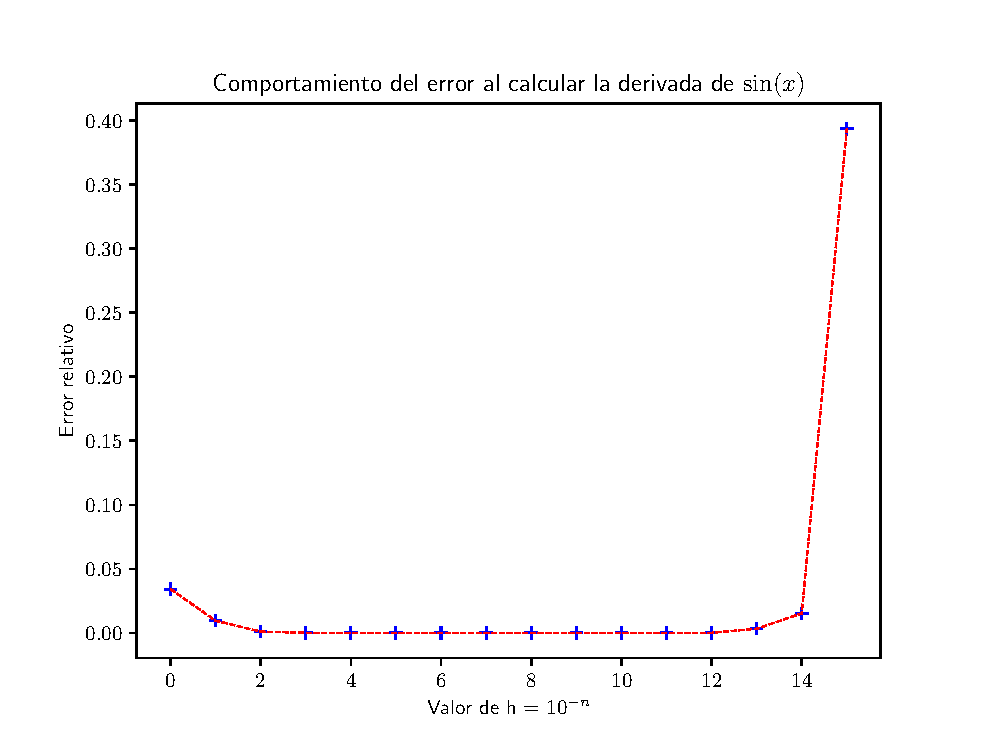
\includegraphics[scale=0.55]{Imagenes/Ejercicio_Derivada_00.eps}
    \caption{Grafica del comportamiento del error relativo en escala normal.}
\end{figure}
\end{frame}
\begin{frame}[fragile]
\frametitle{Ajuste de eje en la gráfica}
Vemos que hay un comportamiento de cambio drástico con los valores del error relativo, donde en apariencia el error relativo se cancela.
\\
\bigskip
\pause
Si ajustamos el eje $y$ a una escala logarítmica, quizá encontremos un resultado interesante.
\end{frame}
\begin{frame}
\frametitle{Gráfica de la tendencia del error}
\begin{figure}
	\centering
    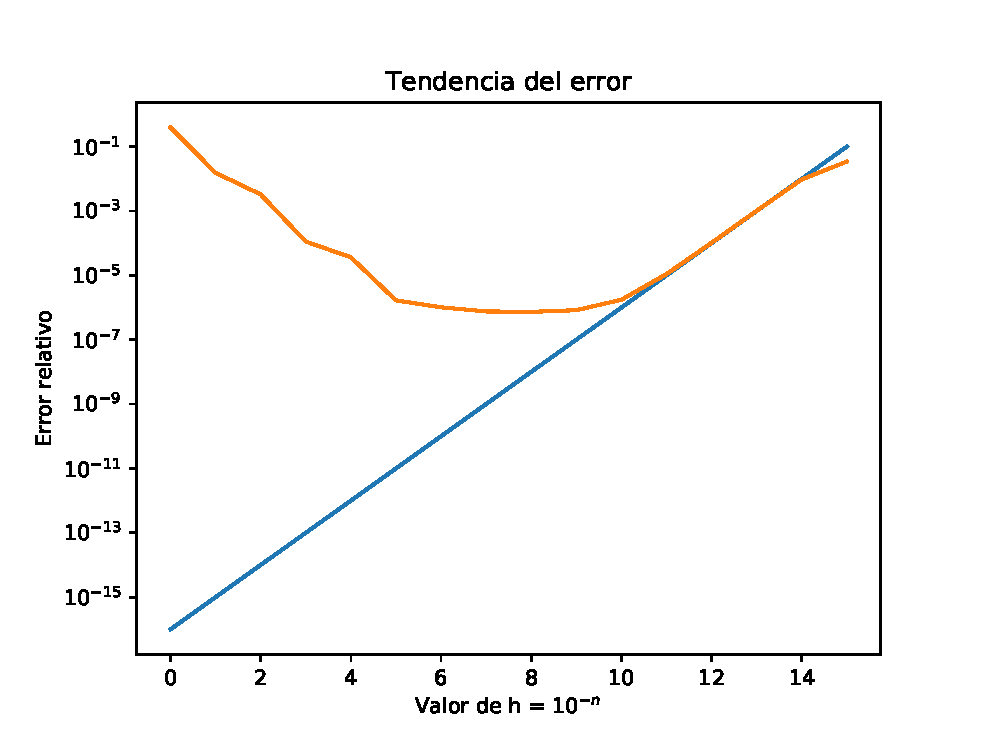
\includegraphics[scale=0.55]{Imagenes/Ejercicio_Derivada_01.eps}
    \caption{Grafica del comportamiento del error relativo en la aproximación.}
\end{figure}
\end{frame}
\begin{frame}
\frametitle{Respuesta a la pregunta}
Si analizamos en detalle, vemos que la tendencia del error de truncamiento es lineal (en escala logarítmica) pero para $h < 10^{-8}$ el error aumenta y no sigue una ley determinada. 
\end{frame}
\begin{frame}
\frametitle{Respuesta a la pregunta}
Este \enquote{empeoramiento} de la aproximación se debe a la incidencia del error de redondeo, es decir, la unidad de máquina pasa a ser más importante que el error de truncamiento.
\end{frame}
\begin{frame}
\frametitle{Respuesta a la pregunta}
Es por eso que no siempre el utilizar una \enquote{mejor precisión} ayuda a mejorar los resultados finales. 
\\
\bigskip
En este tipo de problemas, es conveniente que el error que domine los cálculos sea el de truncamiento o de discretización.
\end{frame}
% \section{Acumulación del error por redondeo}
% \begin{frame}
% Desde que se creó la primera computadora, la acumulación del error de redondeo ha sido uno de los ''dolores de cabeza'' de los especialistas, como se puede ver en esta frase:
% \\
% \medskip
% ''La extraordinaria rapidez de las actuales computadoras significa que en un problema típico se realizan millones de operaciones con coma (punto) flotante. Esto quiere decir que la acumulación de errores de redondeo puede ser desastrosa''.
% \end{frame}
% \begin{frame}
% En muchas ocasiones la inestabilidad está dada por la incidencia de unos pocos errores de redondeo y no por la acumulación de millones de ellos.
% \\
% \medskip
% Un ejemplo en ese sentido está dado por el algoritmo del ejemplo inicial, en el cual el error está dado por el redondeo de $y_{n-1}$, que se propaga a medida que el valor es cada vez más chico.
% \end{frame}
% \begin{frame}
% \frametitle{Ejercicio}
% Calcula el valor de $e$ para $n$ suficientemente grandes, a partir de la su definición:
% \[ f(n) = \lim_{n \rightarrow \infty} \left( 1 + \dfrac{1}{n} \right)^{n} \]
% \end{frame}
% \begin{frame}
% Completa la tabla:
% \begin{center}
% \begin{tabular}{l |l | l}
% n & f(n) & $\vert \exp - f(n) \vert$ \\ \hline
% $10^{1}$ & & \\ \hline
% $10^{2}$ & & \\ \hline
% $10^{3}$ & & \\ \hline
% \ldots & & \\ \hline
% $10^{14}$ & & \\ \hline
% $10^{15}$ & & \\ \hline
% \end{tabular}
% \end{center}
% Discute tus resultados!
% \end{frame}
\end{document}